%%%%%%%%%%%%%%%%%%%%%%%%%%%%%%%%%%%%%%%%%
% Beamer Presentation
% LaTeX Template
% Version 1.0 (10/11/12)
%
% This template has been downloaded from:
% http://www.LaTeXTemplates.com
%
% License:
% CC BY-NC-SA 3.0 (http://creativecommons.org/licenses/by-nc-sa/3.0/)
%
%%%%%%%%%%%%%%%%%%%%%%%%%%%%%%%%%%%%%%%%%

%----------------------------------------------------------------------------------------
%	PACKAGES AND THEMES
%----------------------------------------------------------------------------------------

\documentclass{beamer}

\usepackage{hyperref}

\mode<presentation> {

% The Beamer class comes with a number of default slide themes
% which change the colors and layouts of slides. Below this is a list
% of all the themes, uncomment each in turn to see what they look like.

%\usetheme{default}
%\usetheme{AnnArbor}
%\usetheme{Antibes}
%\usetheme{Bergen}
%\usetheme{Berkeley}
%\usetheme{Berlin}
%\usetheme{Boadilla}
%\usetheme{CambridgeUS}
%\usetheme{Copenhagen}
%\usetheme{Darmstadt}
%\usetheme{Dresden}
%\usetheme{Frankfurt}
%\usetheme{Goettingen}
%\usetheme{Hannover}
%\usetheme{Ilmenau}
%\usetheme{JuanLesPins}
%\usetheme{Luebeck}
\usetheme{Madrid}
%\usetheme{Malmoe}
%\usetheme{Marburg}
%\usetheme{Montpellier}
%\usetheme{PaloAlto}
%\usetheme{Pittsburgh}
%\usetheme{Rochester}
%\usetheme{Singapore}
%\usetheme{Szeged}
%\usetheme{Warsaw}

% As well as themes, the Beamer class has a number of color themes
% for any slide theme. Uncomment each of these in turn to see how it
% changes the colors of your current slide theme.

%\usecolortheme{albatross}
%\usecolortheme{beaver}
%\usecolortheme{beetle}
%\usecolortheme{crane}
%\usecolortheme{dolphin}
%\usecolortheme{dove}
%\usecolortheme{fly}
%\usecolortheme{lily}
%\usecolortheme{orchid}
%\usecolortheme{rose}
%\usecolortheme{seagull}
%\usecolortheme{seahorse}
%\usecolortheme{whale}
%\usecolortheme{wolverine}

%\setbeamertemplate{footline} % To remove the footer line in all slides uncomment this line
%\setbeamertemplate{footline}[page number] % To replace the footer line in all slides with a simple slide count uncomment this line

%\setbeamertemplate{navigation symbols}{} % To remove the navigation symbols from the bottom of all slides uncomment this line
}

\usepackage{graphicx} % Allows including images
\usepackage{booktabs} % Allows the use of \toprule, \midrule and \bottomrule in tables

%----------------------------------------------------------------------------------------
%	TITLE PAGE
%----------------------------------------------------------------------------------------

\title[MT-RT Comparison]{Status of Modtran/LibRadTran simulation and Comparison in december 2016} % The short title appears at the bottom of every slide, the full title is only on the title page

\author{
Dagoret-Campagne, Sylvie  ,  LAL, % Your name
\textit{dagoret@lal.in2p3.fr} % Your email address 
\\
\and
Gilmore, David Kirk , SLAC,
\textit{dkg@slac.stanford.edu} % Your email address
\and
\\
For PCWG team of DESC-LSST collaboration 
}

\date{\today} % Date, can be changed to a custom date

\begin{document}

\begin{frame}
\titlepage % Print the title page as the first slide
\end{frame}

\begin{frame}
\frametitle{Overview} % Table of contents slide, comment this block out to remove it
\tableofcontents % Throughout your presentation, if you choose to use \section{} and \subsection{} commands, these will automatically be printed on this slide as an overview of your presentation
\end{frame}

%----------------------------------------------------------------------------------------
%	PRESENTATION SLIDES
%----------------------------------------------------------------------------------------


%%%%%%%%%%%%%
\section{Reminder on the specifications}
%%%%%%%%%%%%%


%%%%%%%%%%%%%%%
\section{The prescription}
%%%%%%%%%%%%%%%%%

%---------------------------------------------------------------------
% Slide 1
%---------------------------------------------------------------------
\begin{frame}
\frametitle{Data points of the grid}
\begin{block}{Altitude}
$h=2.75$~km.
\end{block}

\begin{block}{Wavelength range}
$\lambda \in [250,1200]$~nm, $\Delta \lambda=$1~nm
\end{block}

\begin{block}{Airmass range}
$z$ computed for 31 points in steps of 0.1~: $z \in [1,3]$
\end{block}

\end{frame}

%---------------------------------------------------------------------
% Slide 2
%---------------------------------------------------------------------

\begin{frame}
\frametitle{The Atmospheric Profile}
Compare predictions for 2 realistic atmospheric models.
\begin{itemize}
\item US standard atmosphere $\rightarrow$ probably good for LSST, but perhaps  a little too wet
\item Subarctic winter $\rightarrow$ very dry air, probably well suited for LSST site
\end{itemize}

\textcolor{gray}{The above atmospheric models are both available in Modtran(Data Card : Card1.MODEL )  and LibRadTran (Data Card : atmosphere\_file.)}

\end{frame}


%---------------------------------------------------------------------
% Slide 3
%---------------------------------------------------------------------

\begin{frame}
\frametitle{Main  absorption models  used in LibRadTran}
\begin{itemize}
\item {\bf Representative wavelengths parameterization (REPTRAN)},
\item {\bf Pseudo-spectral calculation adapted from LOWTRAN}. 
\item {\bf CRS: switching off spectral parameterization}. 
\end{itemize} 
\begin{block} {\bf Absorption models in LibRadTran~:} 
1) REPTRAN, 2) LOWTRAN,  3) CRS, 
\end{block}

\end{frame}


%---------------------------------------------------------------------
% Slide 4
%---------------------------------------------------------------------

\begin{frame}
\frametitle{The absorption models  in Modtran}

\begin{itemize}
\item {\bf Band models methods}, The Modtran or Lowtran models,
\item {\bf The correlated-k method}, The Modtran and Lowtran either in slow or medium modes.
\end{itemize} 

\begin{block} {\bf Absorption models in Modtran~:} 
1) MODTRAN band Model, 2) LOWTRAN Band Model ,  3) MODTRAN correlated-k  and slow speed,  4) MODTRAN correlated-k  and slow speed, 5) MODTRAN correlated-k  and medium speed
\end{block}

\textcolor{gray}{The Data card for specifying the absorption model in Modtran is  \textit{CARD1 MODTRN } . One should provides the values \textit{T,M,C,K,F,L} and \textit{CARD1 SPEED} is \textit{S} or blank. }
\end{frame}



%---------------------------------------------------------------------
% Slide 5
%---------------------------------------------------------------------

\begin{frame}
\frametitle{Different modes : Selected interaction processes}
\begin{itemize}
\item Simulate with only molecular scattering (Rayleigh scattering) (code name \bf{$sc$}). 
\item Simulate pure molecular absorption (code name \bf{$ab$}).
\begin{block}{Variation of Precipitable Pressure Water $PWV$}
 absorption profiles  for 31 points $pwv$ $\in \left[0~{\rm mm},15~{\rm mm} \right]$ in steps of 0.5~mm\end{block}
 \begin{block}{Variation of Ozone $O_3$}
 absorption profiles for  21 points $O_3$ $\in \left[200~{\rm Dobson},600~{\rm Dobson} \right]$.
\end{block}
\item Simulate the combination of molecular scattering and molecular absorption (code name \bf{$sa$}). 
\begin{itemize}
\item perform similar variations in $PWV$ and $O_3$
\end{itemize}
\end{itemize} 
\end{frame}

%----------------------------------------------------------------------------------------------------------------------------------------------

%%%%%%%%%%%%%%%
\section{Practical file organization}
%%%%%%%%%%%%%%%

%---------------------------------------------------------------------
% Slide 6
%---------------------------------------------------------------------
\begin{frame}
\frametitle{File naming : Part 1 }
\begin{block}{filename}
$P\_O\_\{rte\}\_\{atm\}\_\{proc\}\_\{mod\}\_zXX\_wvXX\_ozXX.extension $ 
\end{block}
{\tiny
\begin{itemize}
\item [{\bf P :} ] {\bf RT} or {\bf MT} for LibRadtran or Modtran,
\item [{\bf O :} ]  Observatory site {\bf LS} or {\bf HP}  or {\bf GM}  or {\bf MK} for LSST, OHP, Gemini South, Mauna Kea,...
\item [{\bf \{rte\} :}] {\bf pp} or  {\bf ps},
\item [{\bf \{atm\} :}]  {\bf us} or {\bf sw},
\item [{\bf \{proc\} :}] {\bf sc} for pure molecular scattering, {\bf ab} for pure molecular absorption, {\bf sa} for the combination of molecular scattering and absorption,
\item [{\bf \{mod\} :}] in LibRadTran :  {\bf rt} for Reptran model, {\bf lt} for Lowtran model, {\bf cr} for CRS model,  {\bf fu} for the Fu and Liou model, {\bf k2} for Kato2 model, and {\bf kt} for Kato model.
\item [{\bf \{mod\} :}] in ModTran :  {\bf mt} for Modtran band model), {\bf mk} for Modtran correlated-k model, {\bf lt} for Lowtran model.
\item [{\bf zXX :} ] Airmass $z$, where XX is the value of the airmass on 2 digit $XX=2\times z$,
\item [{\bf wvXX :} ] Precipitable water vapour $pwv$, where XX is the value of the $pwv$ on 3 digit $XXX=10\times pwv$, $pwv$ in mm unit,
\item [{\bf ozXX :} ] Ozone $oz$, where XX is the value of the $oz$ on 2 d igit $XX=oz/10$, $oz$ is Dobson unit.
\end{itemize}

For example a filename for LibRadtran, for LSST could be~:
\begin{equation}
RT\_LS\_pp\_us\_sa\_rt\_z15\_wv030\_oz30.txt  \nonumber
\end{equation}
where $pwv=3$~mm and $oz=300$~Dobson unit and $z=1.5$.

}
\end{frame}

\begin{frame}[fragile]
\frametitle{Example of US standard atmosphere, with Reptran, for airmass $z=1$ and $z=2$, when varying $PWV$ :}
See repository at :
\href{https://github.com/LSSTDESC/PC5AtmosphericExtinction/tree/master/LibRadTran/simulations}{https://github.com/LSSTDESC/PC5AtmosphericExtinction/tree/master/LibRadTran/simulations}
\begin{block}{ls  PC5AtmosphericExtinction/LibRadTran/simulations/RT/2.0/LS/pp/us/ab/rt/wv/out}
{\scriptsize
\begin{verbatim}
RT_LS_pp_us_ab_rt_z10_wv0.OUT	RT_LS_pp_us_ab_rt_z20_wv30.OUT
RT_LS_pp_us_ab_rt_z10_wv10.OUT	RT_LS_pp_us_ab_rt_z20_wv35.OUT
RT_LS_pp_us_ab_rt_z10_wv100.OUT	RT_LS_pp_us_ab_rt_z20_wv40.OUT
RT_LS_pp_us_ab_rt_z10_wv105.OUT	RT_LS_pp_us_ab_rt_z20_wv45.OUT
RT_LS_pp_us_ab_rt_z10_wv110.OUT	RT_LS_pp_us_ab_rt_z20_wv5.OUT
RT_LS_pp_us_ab_rt_z10_wv115.OUT	RT_LS_pp_us_ab_rt_z20_wv50.OUT
RT_LS_pp_us_ab_rt_z10_wv120.OUT	RT_LS_pp_us_ab_rt_z20_wv55.OUT
RT_LS_pp_us_ab_rt_z10_wv125.OUT	RT_LS_pp_us_ab_rt_z20_wv60.OUT
RT_LS_pp_us_ab_rt_z10_wv130.OUT	RT_LS_pp_us_ab_rt_z20_wv65.OUT
RT_LS_pp_us_ab_rt_z10_wv135.OUT	RT_LS_pp_us_ab_rt_z20_wv70.OUT
RT_LS_pp_us_ab_rt_z10_wv140.OUT	RT_LS_pp_us_ab_rt_z20_wv75.OUT
\end{verbatim}
}
\end{block}
\end{frame}
%---------------------------------------------------------------------
% Slide 9
%---------------------------------------------------------------------
\begin{frame}
\frametitle{File naming  : Part 2 }
Naming absorption models for Modtran
\begin{block}{filename}
$P\_O\_\{rte\}\_\{atm\}\_\{proc\}\_\{mod\}\_zXX\_wvXX\_ozXX.extension $ 
\end{block}
{\tiny
\begin{itemize}
\item [{\bf \{mod\} :}] 
{\tiny
\begin{itemize}
{\scriptsize
 \item {\bf mt} for Modtran band model (\textcolor{gray}{CARD1.MODTRN='T'}), 
 \item {\bf mm} for Modtran band model (\textcolor{gray}{CARD1.MODTRN='M'}),, 
 \item {\bf lt} for Lowtran band model (\textcolor{gray}{CARD1.MODTRN='L' or 'F'}), 
 \item {\bf mks} for Modtran correlate-k in slow mode (speed), (\textcolor{gray}{CARD1.MODTRN='K' or 'C and CARD1.SEED='S'}), 
 \item {\bf mkm} for Modtran correlate-k in medium mode (speed), (\textcolor{gray}{CARD1.MODTRN='K' or 'C and CARD1.SEED='M'}),
 }
 \end{itemize}
 }
\end{itemize}
For example a filename for Modtran, for LSST could be~:
\begin{equation}
MT\_LS\_pp\_us\_sa\_mt\_z15\_wv030\_oz30.txt  \nonumber
\end{equation}
where $pwv=3$~mm and $oz=300$~Dobson unit.
}
\end{frame}

%---------------------------------------------------------------------
% Slide 10
%---------------------------------------------------------------------


\begin{frame}
\frametitle{Example of Hierarchy of directories}
\begin{table}
{\tiny
\begin{tabular}{ l l}
  rootdir &  top directory \\
 rootdir/RT/VXX/LS/pp/us/sc/ & pure molecular scattering \\
 rootdir/RT/VXX/LS/pp/us/ab/rt/wv/ & pure molecular absorption for varying $pwv$ \\
 rootdir/RT/VXX/LS/pp/us/ab/rt/oz/ & pure molecular absorption for varying $oz$ \\
 rootdir/RT/VXX/LS/pp/us/sa/rt/wv/ & molecular absorption and scattering for varying $pwv$ \\
 rootdir/RT/VXX/LS/pp/us/sa/rt/oz/ & molecular absorption scattering for varying $oz$ \\
 rootdir/RT/VXX/LS/pp/us/sc/ae/ & pure molecular scattering and default aerosols scattering \\
 rootdir/RT/VXX/LS/pp/us/sa/rt/ae/ & molecular absorption scattering and default aerosols scattering \\
 rootdir/RT/VXX/LS/pp/us/sc/as/ & pure molecular scattering and special aerosols scattering \\
 rootdir/RT/VXX/LS/pp/us/sa/rt/as/ & molecular absorption scattering and special aerosols scattering \\
\end{tabular}
}
\end{table}
{\scriptsize
\begin{itemize}
\item $RT$ means LibRadTran
\item $VXX=2.0$ is the version number of Radtran or Modtran.
\item $LS$ means LSST site,
\item $pp$ means geometry of parallel planes for the atmosphere
\end{itemize}
}
\end{frame}

\section{Example of a comparison inside LibRadTran}
\begin{frame}
\frametitle{Example of  comparison inside LibRadTran : REPTRAN vs LOWTRAN}
\begin{block}{Magnitude calculation}
$F_{\Delta \lambda}^{ADU} =\frac{\pi D^2}{4 g_{el} h c} \int_{\Delta \lambda} T^{atm}(\lambda) T^{filt}(\lambda) \epsilon_{CCD}(\lambda) S^E_\lambda(\lambda) \lambda d\lambda$
\end{block}
\begin{columns}
\begin{column}{0.5\textwidth}
 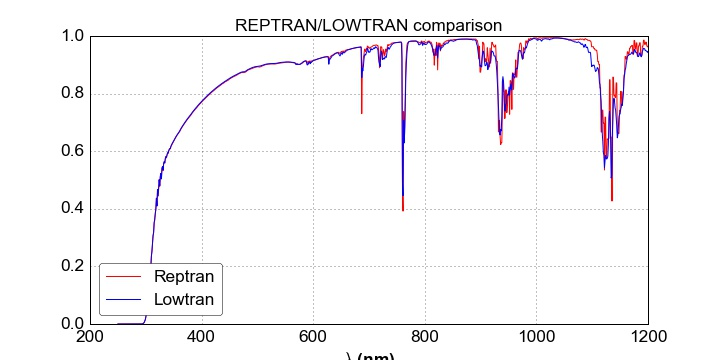
\includegraphics[width=6cm]{images/airtransp.jpg}
\end{column}
\begin{column}{0.5\textwidth}
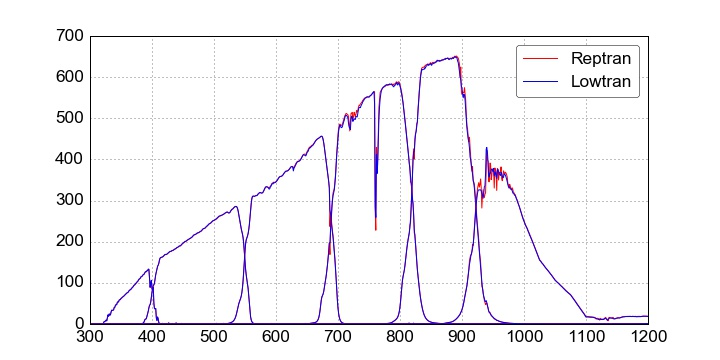
\includegraphics[width=6cm]{images/compmagnit.jpg}      
\end{column}
\end{columns}
\begin{example}
{\scriptsize
For a flat SED~ $S^E_\lambda (\lambda)= cte$, with $z=1$~:
\begin{tabular}{| cc | cc |  cc |}  \hline
filter & mag-shift (mmag) & filter & mag-shift (mmag) & filter & mag-shift (mmag) \\ \hline
U & - 3.0  & I & + 8.9 & G & -2.6  \\
 Z & 7.3  &  R & + 1.5 &  Y4 & 4.5 \\ \hline
\end{tabular}
}
\end{example}
\end{frame}


%---------------------------------------------------------------------
% Slide 11
%---------------------------------------------------------------------

\begin{frame}
\frametitle{Status of the work}
{\tiny
\begin{itemize}
\item GitHub Repository created by Nicolas at \\
 \href{https://github.com/DarkEnergyScienceCollaboration/PC5AtmosphericExtinction}{https://github.com/DarkEnergyScienceCollaboration/PC5AtmosphericExtinction}
\item Prescription note written to proceed with air transparency simulations and posted at \\
 \href{https://github.com/DarkEnergyScienceCollaboration/PC5AtmosphericExtinction/tree/master/doc/Prescriptions}{https://github.com/DarkEnergyScienceCollaboration/PC5AtmosphericExtinction/tree/master/doc/Prescriptions}
\item Simulation with LibRadTran {\bf done} and at posted at (see README) \\
\href{https://github.com/DarkEnergyScienceCollaboration/PC5AtmosphericExtinction/tree/master/LibRadTran/simulations}{https://github.com/DarkEnergyScienceCollaboration/PC5AtmosphericExtinction/tree/master/LibRadTran/simulations}
\item Simulation with Modtran {\bf soon performed} and at posted at (see README) \\
\href{https://github.com/DarkEnergyScienceCollaboration/PC5AtmosphericExtinction/tree/master/ModTran}{https://github.com/DarkEnergyScienceCollaboration/PC5AtmosphericExtinction/tree/master/ModTran}
\end{itemize}
}

\begin{itemize}
\item Ready for Atmospheric properties Analysis,
\item Almost ready for comparison, at least comparing the different models inside LibRadTran.
\end{itemize}

\end{frame}





\begin{frame}
\Huge{\centerline{The End}}

\end{frame}

%----------------------------------------------------------------------------------------

\end{document} 